\section{Hàm số lượng giác và đồ thị}

\subsection{ĐỀ 1}
\Opensolutionfile{ans}[ans/ans-11-C1B4-DE1-LC]
\caulc
\begin{ex}%[1D1N4-2]
%Câu 1
Tìm tập xác định của hàm số $y=\dfrac{1-\sin x}{\cos x}$
\choice
{\True $x\ne \dfrac{\pi }{2}+k\pi, k\in \mathbb{Z} $}
{$x\ne -\dfrac{\pi }{2}+k2\pi, k\in \mathbb{Z} $ }
{$x\ne \dfrac{\pi }{2}+k2\pi, k\in \mathbb{Z}  $}
{$x\ne k\pi, k\in \mathbb{Z}  $}
\loigiai{
Hàm số $y=\dfrac{1-\sin x}{\cos x}$ xác định khi $\cos x\ne 0\Leftrightarrow x\ne \dfrac{\pi }{2}+k\pi $.}
\end{ex}
\begin{ex}%[1D1N4-2]
%Câu 2
Tập xác định của hàm số \( y = \tan 2x \) là
\choice
{\( \mathscr{D} = \mathbb{R}\backslash \left\{ \dfrac{\pi }{4}+k\pi ,k\in \mathbb{Z} \right\} \)}
{\True \( \mathscr{D} = \mathbb{R}\backslash \left\{ \dfrac{\pi }{4}+k\dfrac{\pi }{2},k\in \mathbb{Z} \right\} \)}
{\( \mathscr{D} = \mathbb{R}\backslash \left\{ k\dfrac{\pi }{2},k\in \mathbb{Z} \right\} \)}
{\( \mathscr{D} = \mathbb{R}\backslash \left\{ \dfrac{\pi }{2}+k\pi ,k\in \mathbb{Z} \right\} \)}
\loigiai{
Điều kiện \( \cos 2x \neq 0 \Leftrightarrow 2x \neq \dfrac{\pi }{2}+k\pi \Leftrightarrow x \neq \dfrac{\pi }{4}+k\dfrac{\pi }{2}, k \in \mathbb{Z} \).\\
Vậy tập xác định là \( \mathscr{D} = \mathbb{R}\backslash \left\{ \dfrac{\pi }{4}+k\dfrac{\pi }{2},k\in \mathbb{Z} \right\} \).}
\end{ex}
\begin{ex}%[1D1N4-2]
%Câu 3
Tập xác định của hàm số $y=\dfrac{2\sin x+1}{1-\cos x}$ là
\choice
{\True $\mathscr{D} = \mathbb{R}\backslash\{k2\pi, k\in \mathbb{Z}\}  $}
{$\mathscr{D} = \mathbb{R}\backslash\{ k\pi, k\in \mathbb{Z} \} $}
{$\mathscr{D} = \mathbb{R}\backslash\left\{ \dfrac{\pi }{2}+k\pi, k\in \mathbb{Z} \right\} $}
{$\mathscr{D} = \mathbb{R}\backslash\left\{ \dfrac{\pi }{2}+k2\pi, k\in \mathbb{Z} \right\} $}
\loigiai{
Hàm số xác định khi $1-\cos x\ne 0\Leftrightarrow x\ne k2\pi, k\in \mathbb{Z}$.}
\end{ex}
\begin{ex}%[1D1N4-3]
%Câu 5
Hàm số nào sau đây nghịch biến trên $\left( \dfrac{\pi }{2};\pi \right)$?
\choice
{$y=-\sin x$}
{\True $y=\cos x$}
{$y=-\cot x$}
{$y=\tan x$}
\loigiai{
Với $x\in \left( \dfrac{\pi }{2};\pi \right)$, khi giá trị của $x$ tăng thì giá trị tương ứng của hàm số $y=\cos x$ giảm.\\
$\Rightarrow $ Hàm số $y=\cos x$ nghịch biến trên $\left( \dfrac{\pi }{2};\pi \right)$.}
\end{ex}
\begin{ex}%[1D1N4-3]
%Câu 8
Tìm mệnh đề đúng.
\choice
{Hàm số $y=\cot x$ đồng biến trên khoảng $\left( 0;\pi \right)$}
{\True Hàm số $y=\sin x$ đồng biến trên khoảng $\left( \dfrac{3\pi }{2};\dfrac{5\pi }{2} \right)$}
{Hàm số $y=\sin x$ nghịch biến trên khoảng $\left( \pi ;2\pi \right)$}
{Hàm số $y=\cos x$ nghịch biến trên khoảng $\left( -\dfrac{\pi }{2};\dfrac{\pi }{2} \right)$}
\loigiai{Hàm số $\sin x$ đồng biến trên các khoảng $\left(-\dfrac{\pi}{2}+k2\pi;\dfrac{\pi}{2}+k2\pi\right)(k\in \mathbb{Z})$.}
\end{ex}
\begin{ex}%[1D1N4-4]
%Câu 10
Khẳng định nào dưới đây là \textbf{sai}?
\choice
{\True Hàm số $y=\cos x$ là hàm số lẻ}
{Hàm số $y=\cot x$ là hàm số lẻ}
{Hàm số $y=\sin x$ là hàm số lẻ}
{Hàm số $y=\tan x$ là hàm số lẻ}
\loigiai{
Ta có các kết quả sau:
\begin{itemize}
	\item  Hàm số $y=\cos x$ là hàm số chẵn.
	\item  Hàm số $y=\cot x$ là hàm số lẻ.
	\item  Hàm số $y=\sin x$ là hàm số lẻ.
	\item  Hàm số $y=\tan x$ là hàm số lẻ.
\end{itemize}}
\end{ex}
\begin{ex}%[1D1N4-4]
%Câu 12
Hàm số nào sau đây là hàm số chẵn trên $\mathbb{R}$?
\choice
{$y=x\cdot\cos 2x$}
{$y=\left( x^2+1 \right)\cdot\sin x$}
{\True $y=\dfrac{\cos x}{1+x^2}$}
{ $y=\dfrac{\tan x}{1+x^2}$}
\loigiai{
Xét hàm số $y=f\left( x \right)=\dfrac{\cos x}{1+x^2}$ có tập xác định $\mathscr{D}=\mathbb{R}$
\begin{itemize}
	\item  $\forall x\in \mathscr{D}\Rightarrow -x\in \mathscr{D}$.
	\item  $\forall x\in \mathscr{D}$: $f\left( -x \right)=\dfrac{\cos \left( -x \right)}{1+{{\left( -x \right)}^2}}=\dfrac{\cos x}{1+x^2}=f\left( x \right)$.
\end{itemize}
Vậy hàm số $f$ là hàm chẵn.}
\end{ex}
\begin{ex}%[1D1N4-4]
%Câu 13
Hàm số nào sau đây là hàm số lẻ trên tập xác định của nó?
\choice
{$y=\dfrac{\sin x}{1-\sin x}$}
{ $y=\dfrac{{{\sin }^2}x}{1+\cos x}$}
{$y=\dfrac{\cos x}{x+x^2}$}
{\True $y=\dfrac{\tan x}{1+{{\sin }^2}x}$}
\loigiai{
Xét hàm số $y=f\left( x \right)=\dfrac{\tan x}{1+{{\sin }^2}x}$ có tập xác định $\mathscr{D}=\mathbb{R}\backslash \left\{ \dfrac{\pi }{2}+k\pi \,,\,k\in \mathbb{Z} \right\}$
\begin{itemize}
	\item  $\forall x\in \mathscr{D}\Rightarrow -x\in \mathscr{D}$.
	\item  $\forall x\in \mathscr{D}$: $f\left( -x \right)=\dfrac{\tan \left( -x \right)}{1+{{\sin }^2}\left( -x \right)}=\dfrac{-\tan x}{1+{{\sin }^2}x}=-f\left( x \right)$.
\end{itemize}
Vậy hàm số $f$ là hàm lẻ.}
\end{ex}
\begin{ex}%[1D1N4-5]
%Câu 16
Chọn khẳng định \textbf{sai}.
\choice
{Hàm số $y=\tan \,x+\sin \,x$ là hàm số tuần hoàn với chu kì $2\pi $}
{Hàm số $y=\cos \,x$ là hàm số tuần hoàn với chu kì $2\pi $}
{Hàm số $y=\cot x+\tan x$ là hàm số tuần hoàn với chu kì $\pi $}
{\True Hàm số $y=\sin \,x$ là hàm số tuần hoàn với chu kì $\pi $}
\loigiai{
Hàm số $y=\sin \,x$ và $y=\cos\,x$ tuần hoàn với chu kì $2\pi $.\\
Hàm số $y=\tan \,x$ và $y=\cot\,x$ tuần hoàn với chu kì $\pi $.
}\end{ex}
\begin{ex}%[1D1N4-5]
%Câu 17
Hàm số $y=\sin 2x$ tuần hoàn với chu kỳ bằng bao nhiêu?
\choice
{$T=4\pi $}
{$T=2\pi $}
{\True $T=\pi $}
{$T=\dfrac{\pi }{2}$}
\loigiai{
Hàm số $y=\sin 2x$ tuần hoàn với chu kỳ bằng $T=\dfrac{2\pi }{2}=\pi $.
}\end{ex}
\begin{ex}%[1D1N4-6]
%Câu 20
Tập giá trị của hàm số $y=\cot x$ là
\choice
{$\left( -\infty ;0 \right)$}
{$\left[ -1;1 \right]$}
{$\left( -1;1 \right)$}
{\True $\mathbb{R}$}
\loigiai{Tập giá trị của hàm số $y=\cot x$ là $\mathbb{R}$.}
\end{ex}
\begin{ex}%[1D1N4-6]
%Câu 21
Tìm giá trị lớn nhất của hàm số $y=3\sin \left( x+\dfrac{\pi }{4} \right)-7$
\choice
{$\max y=-7$}
{$\max y=4$}
{$\max y=3$}
{\True $\max y=-4$}
\loigiai{
Ta có $-1\le \sin \left( x+\dfrac{\pi }{4} \right)\le 1\Rightarrow -10\le y\le -4$. Do đó $\max y=-4$.}
\end{ex}
\Closesolutionfile{ans}
\indapan{6}{ans/ans-11-C1B4-DE1-LC}

\Opensolutionfile{ans}[ans/ans-11-C1B4-DE1-DS]
\cauds
%%%==============EX_1============%%%
\begin{ex}
	Cho hàm số $f(x)=\tan 2x-1$. Khi đó:
	\choiceTF
		{\True Giá trị của hàm số tại $x=\dfrac{\pi}{8}$ bằng $0$}
		{\True Giá trị của hàm số tại $x=\dfrac{\pi}{3}$ bằng $-\sqrt{3}-1$}
		{Có ba giá trị $x$ thuộc $[0;\pi]$ khi hàm số đạt giá trị bằng $-2$}
		{\True Hàm số đã cho là hàm tuần hoàn}
	\loigiai{
	\begin{itemchoice}
			\itemch Đúng. Ta có
			$f\left(\dfrac{\pi}{8} \right)=\tan \left(2\cdot \dfrac{\pi}{8} \right)-1=1-1=0$.
			 \itemch Đúng. Ta có $f\left(\dfrac{\pi}{3} \right)=\tan \left(2\cdot \dfrac{\pi}{3} \right)-1=-\sqrt{3}-1$.
			\itemch Sai. Ta có 
$$
\begin{aligned}
f(x)=-2&\Leftrightarrow \tan 2x-1=-2\Leftrightarrow \tan 2x=-1\\
		&\Leftrightarrow 2x=-\dfrac{\pi}{4}+k\pi (k\in \mathbb{Z})\Leftrightarrow x=-\dfrac{\pi}{8}+k\dfrac{\pi}{2} (k\in \mathbb{Z}).
\end{aligned}
$$					
			Vì $x\in [0;\pi]$ nên $x\in \left\{\dfrac{3\pi}{8};\dfrac{7\pi}{8} \right\}$ (khi đó $k=1;k=2$).
			\itemch Đúng. Tập xác định hàm số là $\mathscr{D}=\mathbb{R}\setminus \left\{\dfrac{\pi}{4}+k\dfrac{\pi}{2} k\in \mathbb{Z}\right\}$.
			
			Với mọi $x\in \mathscr{D}$, ta có $x\pm \dfrac{\pi}{2} \in \mathscr{D}$ và
			\[f\left(x+\dfrac{\pi}{2} \right)=\tan 2\left(x+\dfrac{\pi}{2} \right)-1=\tan (2x+\pi)-1=\tan 2x-1=f(x).
			\]
			Vậy hàm số đã cho là hàm tuần hoàn.
		\end{itemchoice}
}
\end{ex}
%%%==============EX_2============%%%
\begin{ex}
	Cho hàm số $f(x)=\sin^2 x+\cos x-1$. Khi đó:
	\choiceTF
		{\True Tập xác định của hàm số $\mathscr{D}=\mathbb{R}$}
		{$f(-\pi)=-f(\pi)$}
		{\True $f(-x)=f(x)$}
		{\True Hàm số đã cho là hàm số chẵn}
	\loigiai{
	\begin{itemchoice}
		\itemch	Đúng. Tập xác định của hàm số $\mathscr{D}=\mathbb{R}$. 
		\itemch	Sai. Với mọi $x\in \mathscr{D}$, ta có
		$$-x\in \mathscr{D} \text{ và }f(-x)=\sin^2 (-x)+\cos (-x)-1=\sin^2 x+\cos x-1=f(x).$$
		Vậy hàm số đã cho là hàm số chẵn trên $\mathbb{R}$.
		\itemch Đúng. Vì $f(x)$ là hàm số đã cho là hàm số chẵn trên $\mathbb{R}$.
		\itemch Đúng. Vì $f(x)$ là hàm số đã cho là hàm số chẵn trên $\mathbb{R}$.
	\end{itemchoice}
		}
\end{ex}
%%%==============EX_7============%%%
\begin{ex}
	Tìm được tập giá trị các hàm số sau trên tập xác định của chúng:
	\choiceTF
		{\True Hàm số $y=3\sin x$ có tập giá trị là $T=[-3;3]$}
		{\True Hàm số $y=2\cos x-1$ có tập giá trị là $T=[-3;1]$}
		{\True Hàm số $y=2030-4\cos x$ có tập giá trị là $T=[2026;2034]$}
		{Hàm số $y=\sin^2 x+4\sin x-1$ có tập giá trị là $T=[-3;3]$}
	\loigiai{
	\begin{itemchoice}
		\itemch Đúng. Với mọi $x\in \mathbb{R}$, ta có $-1\le \sin x\le 1\Rightarrow-3\le 3\sin x\le 3\Rightarrow-3\le y\le 3$.
			
			Vậy tập giá trị của hàm số là $T=[-3;3]$.
		\itemch Đúng. Với mọi $x\in \mathbb{R}$, ta có $-1\le \cos x\le 1\Rightarrow-2\le 2\cos x\le 2$ $\Rightarrow-2-1\le 2\cos x-1\le 2-1\Rightarrow-3\le y\le 1$.
			
			Vậy tập giá trị của hàm số là $T=[-3;1]$.
		\itemch Đúng. Với mọi $x\in \mathbb{R}$, ta có $-1\le \cos x\le 1\Rightarrow 4\ge-4\cos x\ge-4$ $\Rightarrow 4+2030\ge-4\cos x+2030\ge-4+2030\Rightarrow 2034\ge y\ge 2026$.
			
			Vậy tập giá trị của hàm số là $T=[2026;2034]$.
		\itemch Sai. Vì $y=\sin^2 x+4\sin x-1=\sin^2 x+4\sin x+4-5=(\sin x+2)^2-5$.
			
			Với mọi $x\in \mathbb{R}$, ta có $-1\le \sin x\le 1\Rightarrow 1\le \sin x+2\le 3$
			\[\Rightarrow 1^2 \le (\sin x+2)^2 \le 3^2 \Rightarrow 1^2-5\le (\sin x+2)^2-5\le 3^2-5\Rightarrow-4\le y\le 4.
			\]
			Vậy tập giá trị của hàm số là $T=[-4;4]$.
		\end{itemchoice}
			}
\end{ex}
%%%==============EX_10============%%%
\begin{ex}
	Cho hàm số $f(x)=2\cos x+1$ và $g(x)=\sin x+\tan x$. Khi đó:
	\choiceTF
		{\True Tập xác định hàm số $f(x)$: $\mathscr{D}=\mathbb{R}$}
		{\True Hàm số $f(x)$ là hàm tuần hoàn}
		{Tập xác định hàm số $g(x)$: $\mathscr{D}=\mathbb{R}\setminus \left\{\dfrac{\pi}{3}+k\pi \left|k\in \mathbb{Z}\right. \right\}$}
		{Hàm số $g(x)$ là hàm không tuần hoàn}
	\loigiai{
	\begin{itemchoice}
		\itemch Đúng. Tập xác định hàm số $\mathscr{D}=\mathbb{R}$.
			
		\itemch	Đúng. Với mọi $x\in \mathscr{D}$ thì $x\pm 2\pi \in \mathscr{D}$ và $f(x+2\pi)=2\cos (x+2\pi)+1=2\cos x+1=f(x)$.
			
			Vậy hàm số đã cho là hàm tuần hoàn.
		\itemch Sai. Tập xác định hàm số $\mathscr{D}=\mathbb{R}\setminus \left\{\dfrac{\pi}{2}+k\pi \left|k\in \mathbb{Z}\right. \right\}$.
			
		\itemch	Sai. Với mọi $x\in \mathscr{D}$ thì $x\pm 2\pi \in \mathscr{D}$ và $$f(x+2\pi)=\sin (x+2\pi)+\tan (x+2\pi)=\sin x+\tan x=f(x).$$
			Vậy hàm số đã cho là hàm tuần hoàn.
	\end{itemchoice}
			}
\end{ex}
\Closesolutionfile{ans}
\indapan{3}{ans/ans-11-C1B4-DE1-DS}

\Opensolutionfile{ans}[ans/ans-11-C1B4-DE1-KQ]
\caukq
%%%==============EX_1============%%%
\begin{ex}%[1D1H4-6]
Tập giá trị của hàm số $y=5+4\sin 2x\cos 2x$ có dạng $[m;M]$. Tìm giá trị $M-m$.
	
	\shortans{$4$}
\loigiai{
	\[y=5+4\sin 2x\cos 2x.
	\]
	Hàm số có tập xác định $\mathscr{D}=\mathbb{R}$.\\
	Ta có $y=5+4\sin 2x\cos 2x=5+2\sin 4x$.\\
	Do $-1\le \sin 4x\le 1\Leftrightarrow-2\le 2\sin 4x\le 2\Leftrightarrow 3\le 5+2\sin 4x\le 7\Leftrightarrow 3\le y\le 7$.\\
	Vậy giá trị của hàm số là $T=[3;7]$. Vậy $M=7$ và $m=3$ nên $M-m=4$.
	}
\end{ex}
%%%==============EX_3============%%%
\begin{ex}%[1D1H4-6]
Tập giá trị của hàm số: $y=\sin x+\sqrt{3} \cos x+3$ có dạng $[m;M]$. Tìm giá trị $M\cdot m$.
	
	\shortans{$5$}
\loigiai{
	\[y=\sin x+\sqrt{3} \cos x+3
	\]
	Ta có $y=\sin x+\sqrt{3} \cos x+3=2\left(\dfrac{1}{2} \sin x+\dfrac{\sqrt{3}}{2} \cos x\right)+3=2\sin \left(x+\dfrac{\pi}{3} \right)+3$.\\
	Do 
	$$
\begin{aligned}
-1\le \sin \left(x+\dfrac{\pi}{3} \right)\le 1&\Leftrightarrow-2\le 2\sin \left(x+\dfrac{\pi}{3} \right)\le 2\\
&\Leftrightarrow 1\le 2\sin \left(x+\dfrac{\pi}{3} \right)+3\le 5\Leftrightarrow 1\le y\le 5.
\end{aligned}
$$
	Vậy giá trị của hàm số là $T=[1;5]$. Vậy $M=5$ và $m=1$ nên $M\cdot m=5$.
	}
\end{ex}
%%%==============EX_5============%%%
\begin{ex}%[1D1H4-6]
Tập giá trị của hàm số: $y=\sin x$ trên đoạn $\left[-\dfrac{\pi}{3};\dfrac{2\pi}{3} \right]$ có dạng $[m;M]$. Tìm giá trị $M^2+m^2$.
	
	\shortans{$1,75$}
\loigiai{
	$y=\sin x$ trên đoạn $\left[-\dfrac{\pi}{3};\dfrac{2\pi}{3} \right]$.\\
	Ta có đồ thị của hàm số $y=\sin x$ trên $\mathbb{R}$ như sau
	\begin{center}
				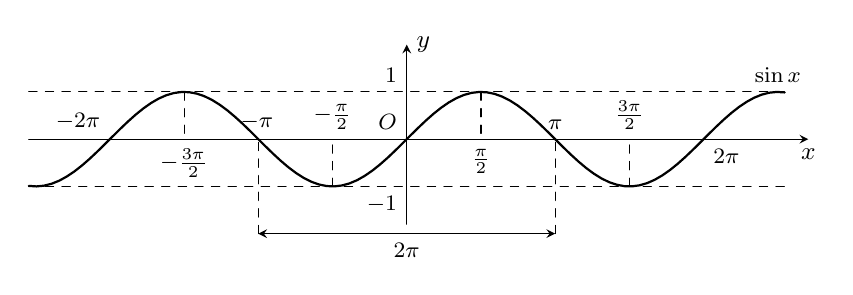
\begin{tikzpicture}[>=stealth,line join=round,line cap=round,font=\footnotesize,scale=0.6]
					\draw[->] (-8,0) -- (8.5,0) node[below] {\small $x$};
					\draw[->] (0,-1.8) -- (0,2) node[right] {\small $y$};
					\draw[thick,samples=100,domain=-8:8] plot(\x,{sin((\x)*180/pi)});
					\draw (0,0) node [above left] {$O$};
					\draw (0,1) node [above left] {$1$};
					\draw (0,-1) node [below left] {$-1$};
					\draw (-2*pi,0) node[above left] {$-2\pi$};
					\draw (2*pi,0) node[below right] {$2\pi$};
					\draw[dashed] (-3*pi/2,1)--(-3*pi/2,0) node[below] {$-\frac{3\pi}{2}$};
					\draw[dashed] (3*pi/2,-1)--(3*pi/2,0) node[above] {$\frac{3\pi}{2}$};
					\draw (-3.17,0) node[above] {$-\pi$};
					\draw (pi,0) node[above] {$\pi$};
					\draw[dashed] (-pi/2,-1)--(-pi/2,0) node[above] {$-\frac{\pi}{2}$};
					\draw[dashed] (pi/2,1)--(pi/2,0) node[below] {$\frac{\pi}{2}$};
					\draw[dashed] (-8,1)--(8,1);
					\draw[dashed] (-8,-1)--(8,-1);
					\draw[<->] (-pi,-2)--(0,-2)node[below] {$2\pi$}--(pi,-2);
					\draw[dashed] (-pi,-2)--(-pi,0);
					\draw[dashed] (pi,-2)--(pi,0);
					\draw (5*pi/2,1) node[above] {$\sin x$};
				\end{tikzpicture}
			\end{center}
	Dựa vào đồ thị trên, ta có bảng biến thiên của hàm số $y=\sin x$ xét trên đoạn $\left[-\dfrac{\pi}{3};\dfrac{2\pi}{3} \right]$
\begin{center}
\begin{tikzpicture}
 \tkzTabInit[lgt=2,espcl=2]
 {$x$ / 1 , $\sin(x)$ / 2 }
 {$\dfrac{-\pi}{3}$, $0$, $\dfrac{\pi}{2}$, $\dfrac{2\pi}{3}$}
 \tkzTabVar{ -/$\frac{-\sqrt{3}}{2}$, R/ , +/$1$, -/$\frac{\sqrt{3}}{2}$}
 \tkzTabIma{1}{3}{2}{0}
\end{tikzpicture}
\end{center}
	Dựa vào bảng biến thiên, ta thấy tập giá trị của hàm số là $T=\left[-\dfrac{\sqrt{3}}{2};1\right]$. Vậy $M=1$ và $m=\dfrac{\sqrt{3}}{2}$ nên $M^2+m^2=1,75$.
	}
\end{ex}
%%%==============EX_8============%%%
\begin{ex}%[1D1H4-6]
Tìm tổng giá trị lớn nhất và giá trị nhỏ nhất của hàm số $y=\dfrac{2\sin x+3\cos x+1}{\sin x-\cos x+2}$.
	
	\shortans{$3$}
\loigiai{
	Ta có $y=\dfrac{2\sin x+3\cos x+1}{\sin x-\cos x+2} \Leftrightarrow (y-2)\sin x-(y+3)\cos x=1-2y$.\\
	Điều kiện để tồn tại cặp số $(x;y)$ là 
	\[(y-2)^2+(y+3)^2 \ge (1-2y)^2\Leftrightarrow-2y^2+6y+12\ge 0\Leftrightarrow \dfrac{3-\sqrt{33}}{2} \le y\le \dfrac{3+\sqrt{33}}{2}.
	\]
	Tổng giá trị lớn nhất và giá trị nhỏ nhất của hàm số: $\dfrac{3-\sqrt{33}}{2}+\dfrac{3+\sqrt{33}}{2}=3$.
	}
\end{ex}
%%%==============EX_9============%%%
\begin{ex}%[1D1H4-6]
Tìm giá trị lớn nhất $(\max y)$ của hàm số $y=\sin^2 x+\sin x-3$.
	
	\shortans{$-1$}
\loigiai{
	Đặt $t=\sin x,t\in [-1;1]$. Ta có $y=t^2+t-3$.\\
	Đây là hàm bậc hai với $a=1,b=1\Rightarrow-\dfrac{b}{2a}=-\dfrac{1}{2}$. Vì $a > 0$ nên bề lõm parabol tương ứng sẽ hướng lên trên.\\
	Bảng biến thiên:
	\begin{center}
	\begin{tikzpicture}[arrow/.style={>=stealth,->,shorten <= 10pt,shorten >= 10pt},font=\footnotesize,xscale=1,yscale=0.5]
			\foreach \i in {0,1,...,9}
			\foreach \j in {1,2,...,9} \coordinate (\i\j)at(\i,\j);
			\draw[thick] ([xshift=-0.5cm,yshift=-1cm]01)rectangle([xshift=0.5cm,yshift=1cm]99) ([xshift=0.5cm,yshift=-1cm]01)--([xshift=0.5cm,yshift=1cm]09) ([xshift=-0.5cm,yshift=-1cm]09)--([xshift=0.5cm,yshift=-1cm]99);
			\draw (09)node{$x$}(05)node{$f(x)$};
			\foreach \nhan/\vtri in {$-\infty$/1,$-1$/3,$-\dfrac{1}{2}$/5,$1$/7,$+\infty$/9}
			\draw (\vtri9)node{\nhan};
			\draw[arrow] (17)--(34);
			\draw[arrow] (34)--(51);
			\draw[arrow] (51)--(74);
			\draw[arrow] (74)--(97);
			\foreach \shf/\nhan/\vtri in {0cm/$+\infty$/17,0cm/$-3$/34,0cm/$-\dfrac{13}{4}$/51,0cm/$-1$/74,0cm/$-\infty$/97}
			\draw ([xshift=\shf]\vtri)node{\nhan};
			\fill [draw, pattern = north west lines](0.5,0)--(0.5,8)--(2.8,8)--(2.8,0)--cycle;
			\fill [draw, pattern = north west lines](7.2,0)--(7.2,8)--(9.5,8)--(9.5,0)--cycle;
		\end{tikzpicture}
	\end{center}
	Dựa vào bảng biến thiên, ta thấy $\max y=-1$, khi đó $t=1\Leftrightarrow \sin x=1$ $\Leftrightarrow x=\dfrac{\pi}{2}+k2\pi (k\in \mathbb{Z})$.
	}
\end{ex}
%%%==============EX_11============%%%
\begin{ex}%[1D1V4-8]
Số giờ có ánh sáng của thành phố $T$ ở vĩ độ $40^{^\circ}$ bắc trong ngày thứ $t$ của một năm không nhuận được cho bởi hàm số $d(t)=3\cdot \sin \left[\dfrac{\pi}{182} (t-80)\right]+12$ với $t\in \mathbb{Z}$ và $0< t\le 365$. Bạn An muốn đi tham quan thành phố $T$ nhưng lại không thích ánh sáng mặt trời, vậy bạn An nên chọn đi vào ngày nào trong năm để thành phố $T$ có ít giờ có ánh sáng mặt trời nhất?
	\shortans{$353$}
\loigiai{
	Do 
$$
\begin{aligned}
\sin \left[\dfrac{\pi}{182} (t-80)\right]\ge-1 &\Rightarrow 3\cdot \sin \left[\dfrac{\pi}{182} (t-80)\right]\ge-3\\
	&\Rightarrow 3\cdot \sin \left[\dfrac{\pi}{182} (t-80)\right]+12\ge 9\Rightarrow d(t)\ge 9.
\end{aligned}
$$	
	Vậy thành phố $T$ có ít giờ có ánh sáng mặt trời nhất khi và chỉ khi:
	\[\sin \left[\dfrac{\pi}{182} (t-80)\right]=-1\Leftrightarrow \dfrac{\pi}{182} (t-80)=-\dfrac{\pi}{2}+k2\pi
	\]
	
	\[\Leftrightarrow t-80=182\left(-\dfrac{1}{2}+2k\right)\Leftrightarrow t=364k-11,k\in \mathbb{Z}.
	\]
	Mặt khác $0\le 364k-11\le 365\Leftrightarrow \dfrac{11}{364} \le k\le \dfrac{376}{364} \Leftrightarrow k=1($ do $k\in \mathbb{Z})$. Nên
	\[ t=364-11=353\]
	Vậy thành phố $T$ có ít giờ ánh sáng Mặt Trời nhất là $9$ giờ khi $t=353$, tức là vào ngày thứ $353$ trong năm.
	}
\end{ex}
\Closesolutionfile{ans}
\indapan{3}{ans/ans-11-C1B4-DE1-KQ}
\subsection{ĐỀ 2}
\Opensolutionfile{ans}[ans/ans-11-C1B4-DE2-LC]
\caulc
\begin{ex}%[1D1N4-6]
%Câu 24
Tìm tập giá trị của hàm số $y=\sin x-1$
\choice
{$\left[ 0;1 \right]$}
{$\left[ -1;0 \right]$}
{\True $\left[ -2;0 \right]$}
{$\left[ 2;0 \right]$}
\loigiai{
Ta có $-1\le \sin x\le 1\Leftrightarrow -2\le \sin x-1\le 0\Leftrightarrow -2\le y\le 0$.\\
Vậy tập giá trị của hàm số $y=\sin x-1$ là $T=\left[ -2;0 \right]$.}
\end{ex}
\begin{ex}%[1D1H4-7]
%Câu 29
Cho đồ thị hàm số $f\left( x \right)$ như hình vẽ dưới đây. Hỏi tịnh tiến đồ thị hàm số $f\left( x \right)$ theo vectơ $\vec{v}=\left( \dfrac{\pi }{2};0 \right)$ thì được đồ thị hàm số
\begin{center}
				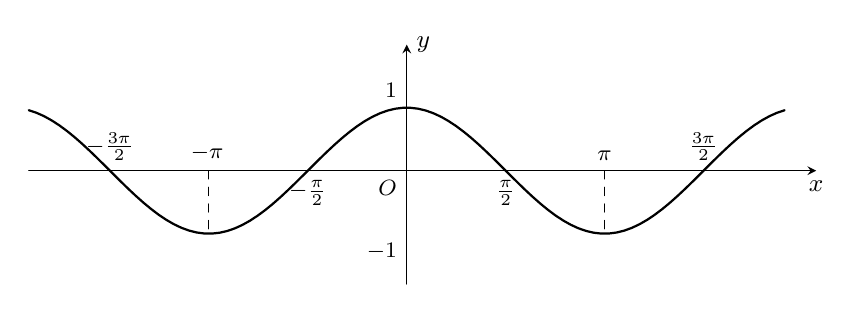
\begin{tikzpicture}[>=stealth,line join=round,line cap=round,font=\footnotesize,scale=0.8]
					\draw[->] (-6,0) -- (6.5,0) node[below] {\small $x$};
					\draw[->] (0,-1.8) -- (0,2) node[right] {\small $y$};
					\draw[thick,samples=100,domain=-6:6] plot(\x,{cos((\x)*180/pi)});
					\draw (0,0) node [below left] {$O$};
					\draw (0,1) node [above left] {$1$};
					\draw (0,-1) node [below left] {$-1$};
					\draw (-4.71,0) node[above] {$-\frac{3\pi}{2}$};
					\draw (4.71,0) node[above] {$\frac{3\pi}{2}$};
					\draw (-3.17,0) node[above] {$-\pi$};
					\draw (pi,0) node[above] {$\pi$};
					\draw[dashed] (-1.57,0) node[below] {$-\frac{\pi}{2}$};
					\draw[dashed] (1.57,0) node[below] {$\frac{\pi}{2}$};
					\draw[dashed] (pi,0)--(pi,-1);
					\draw[dashed] (-pi,0)--(-pi,-1);
				\end{tikzpicture}
			\end{center}
\choice
{$y=\tan x$}
{\True $y=\sin x$}
{$y=\cos x$}
{$y=\cot x$}
\loigiai{
Theo hình vẽ thì đồ thị trong hình là của hàm số $y=\cos x$. Khi tịnh tiến theo vectơ $\vec{v}=\left( \dfrac{\pi }{2};0 \right)$ thì ta được đồ thị của hàm số $y=\cos \left( x-\dfrac{\pi }{2} \right)=\sin x$.}
\end{ex}
\begin{ex}%[1D1H4-7]
%Câu 30
Đường cong trong hình dưới đây là đồ thị của một hàm số trong bốn hàm số được liệt kê ở bốn phương án $A,\ B,\ C,\ D$
 \begin{center}
				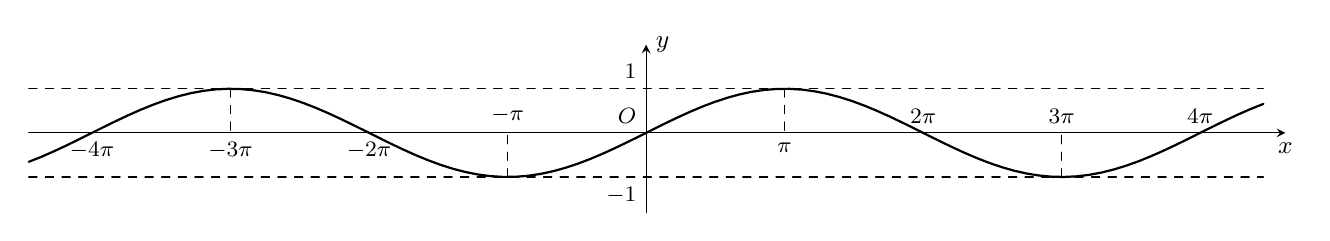
\begin{tikzpicture}[>=stealth,line join=round,line cap=round,font=\footnotesize,scale=0.56]
					\draw[->] (-14,0) -- (14.5,0) node[below] {\small $x$};
					\draw[->] (0,-1.8) -- (0,2) node[right] {\small $y$};
					\draw[thick,samples=100,domain=-14:14] plot(\x,{sin((\x)*90/pi)});
					\draw (0,0) node [above left] {$O$};
					\draw (0,1) node [above left] {$1$};
					\draw (0,-1) node [below left] {$-1$};
					\draw (-2*pi,0) node[below] {$-2\pi$};
					\draw (2*pi,0) node[above] {$2\pi$};
					\draw (-4*pi,0) node[below] {$-4\pi$};
					\draw (4*pi,0) node[above] {$4\pi$};
					\draw[dashed] (-pi,-1)--(-pi,0) node[above] {$-\pi$};
					\draw[dashed] (pi,1)--(pi,0) node[below] {$\pi$};
					\draw[dashed] (-3*pi,1)--(-3*pi,0) node[below] {$-3\pi$};
					\draw[dashed] (3*pi,-1)--(3*pi,0) node[above] {$3\pi$};
					\draw[dashed] (-14,1)--(14,1);
					\draw[dashed] (-14,-1)--(14,-1);
				\end{tikzpicture}
			\end{center}
Hỏi hàm số đó là hàm số nào?
\choice
{$y=\sin \dfrac{x}{2}$}
{$y=\cos \dfrac{x}{2}$}
{$y=-\cos \dfrac{x}{4}$}
{\True $y=\sin \left( -\dfrac{x}{2} \right)$}
\loigiai{
Đồ thị hàm số đi qua điểm $\left( \pi ;-1 \right)$ nên ta chọn hàm số $y=\sin \left( -\dfrac{x}{2} \right)$.}
\end{ex}
\begin{ex}%[1D1N4-7]
%Câu 32
Đồ thị của hàm số $y=\sin \left( x+\dfrac{\pi }{4} \right)$ đi qua điểm nào sau đây?
\choice
{$M\left( \dfrac{\pi }{4}\,;\,0 \right)$ }
{\True $N\left( 0\,;\,\dfrac{\sqrt{2}}{2} \right)$ }
{ $P\left( \dfrac{\pi }{2}\,;\,1 \right)$}
{$Q\left( 0\,;\,1 \right)$}
\loigiai{
Với $x=0\Rightarrow y=\sin \dfrac{\pi }{4}=\dfrac{\sqrt{2}}{2}$.}
\end{ex}
\begin{ex}%[1D1H4-2]
%Câu 33
Cho các hàm số sau\\
(I) $y=-x^3+3x-4$\quad(II) $y=-x^4+3x-4+\dfrac{x+1}{x^2+1}$\\
(III) $y=\sin x$ \qquad(IV) $y=\tan x+\cot x$\\
Có bao nhiêu hàm số có tập xác định là $\mathbb{R}$?
\choice
{$2$}
{$4$}
{$1$}
{\True $3$}
\loigiai{
\begin{itemize}
	\item  Hàm số $y=-x^3+3x-4$ là hàm đa thức nên có tập xác định là $\mathbb{R}$.
	\item  Do $x^2+1>0,\forall x\in \mathbb{R}$ nên hàm số $y=-x^4+3x-4+\dfrac{x+1}{x^2+1}$ có tập xác định là $\mathbb{R}$.
	\item  Hàm số $y=\sin x$ có tập xác định là $\mathbb{R}$.
	\item  Hàm số $y=\tan x+\cot x$ xác định khi và chỉ khi $$\left\{ \begin{aligned}
	& \sin x\ne 0 \\
	& \cos x\ne 0 \\
\end{aligned} \right. \Leftrightarrow \sin 2x\ne 0\Leftrightarrow x\ne k\dfrac{\pi }{2}\left( k\in \mathbb{Z} \right).$$
Nên hàm số $y=\tan x+\cot x$ có tập xác định là $\mathscr{D}=\mathbb{R}\backslash \left\{ \left. k\dfrac{\pi }{2} \right|k\in \mathbb{Z} \right\}$.
	\end{itemize}
Vậy có $3$ hàm số có tập xác định là $\mathbb{R}$.}
\end{ex}
\begin{ex}%[1D1N4-2]
%Câu 35
Tìm tập xác định $\mathscr{D}$ của hàm số $y=\dfrac{2019}{\sin x}$
\choice
{$\mathscr{D}=\mathbb{R}\backslash \left\{ \dfrac{\pi }{2}+k\pi ,k\in \mathbb{Z} \right\}$}
{$\mathscr{D}=\mathbb{R}$}
{$\mathscr{D}=\mathbb{R}\backslash \left\{ 0 \right\}$ }
{\True $\mathscr{D}=\mathbb{R}\backslash \left\{ k\pi ,k\in \mathbb{Z} \right\}$}
\loigiai{
Hàm số xác định khi $\sin x\ne 0\Leftrightarrow x\ne k\pi \left( k\in \mathbb{Z} \right)$.\\
Tập xác định $\mathscr{D}=\mathbb{R}\backslash \left\{ k\pi ,k\in \mathbb{Z} \right\}$.}
\end{ex}
\begin{ex}%[1D1N4-3]
%Câu 40
Xét hàm số $y=\sin x$ trên đoạn $\left[ -\pi ;0 \right]$. Khẳng định nào sau đây là đúng?
\choice
{\True Hàm số đã cho nghịch biến trên đoạn $\left[ -\pi ;-\dfrac{\pi }{2} \right]$; đồng biến trên đoạn $\left[ -\dfrac{\pi }{2};0 \right]$}
{Hàm số đã cho nghịch biến trên các đoạn $\left[ -\pi ;-\dfrac{\pi }{2} \right]$ và $\left[ -\dfrac{\pi }{2};0 \right]$}
{Hàm số đã cho đồng biến trên các đoạn $\left[ -\pi ;-\dfrac{\pi }{2} \right]$ và $\left[ -\dfrac{\pi }{2};0 \right]$}
{Hàm số đã cho đồng biến trên đoạn $\left[ -\pi ;-\dfrac{\pi }{2} \right]$; nghịch biến trên đoạn $\left[ -\dfrac{\pi }{2};0 \right]$}
\loigiai{
Ta có bảng biến thiên của hàm số $y=\sin x$ trên đoạn $\left[ -\pi ;\pi \right]$.
\begin{center}
	\begin{tikzpicture}[font=\normalsize]
	\tkzTabInit[espcl=2]
		{$x$ /1,$g(x)$/2}
		{$-\infty$,$-1$,$1$,$2$,$+\infty$}
	\tkzTabVar{+/$0$,-/$-1$, R /,+/$1$,-/$0$}
	\tkzTabIma{2}{4}{3}{$0$}
\end{tikzpicture}
\end{center}	
Khi đó, hàm số nghịch biến trên đoạn $\left[ -\pi ;-\dfrac{\pi }{2} \right]$; đồng biến trên đoạn $\left[ -\dfrac{\pi }{2};0 \right]$.}
\end{ex}
\begin{ex}%[1D1H4-4]
%Câu 49
Trong các hàm số sau đây, hàm số nào có đồ thị đối xứng qua trục tung?
\choice
{$y=\tan x$}
{\True $y=\cos x$}
{$y=\sin x$}
{$y=\cot x$}
\loigiai{
Hàm số $y=\cos x$ là hàm số chẵn nên có đồ thị đối xứng qua trục tung.}
\end{ex}
\begin{ex}%[1D1H4-5]
%Câu 50
Mệnh đề nào sau đây \textbf{sai}?
\choice
{Hàm số xác định trên tập số thực là hàm số $y=\dfrac{\cos x+\sin x+3}{\sin 3x+\cos 3x+3}$}
{\True Hàm số lượng giác là hàm tuần hoàn với chu kỳ $2\pi $}
{Hàm số có chu kỳ là $\pi $ là hàm số $y=\sin 2x+\tan x+{{\cos }^2}x$}
{Phương trình $\tan x=\sqrt{3}$ có $2$ nghiệm thuộc vào $\left( -3;3 \right)$}
\loigiai{
Phương trình $\sin 3x+\cos 3x+3=0$ vô nghiệm nên hàm số có tập xác định là $\mathbb{R}$.\\
Hàm $y=\tan x$ có chu kỳ là $\pi $.\\
Hàm số $y=\sin 2x+\tan x+{{\cos }^2}x$ có chu kỳ là $\pi $.\\
Phương trình $\tan x=\sqrt{3}$ có $2$ nghiệm $x=\pm \dfrac{\pi }{3}$ thuộc khoảng $\left( -3;3 \right)$.}
\end{ex}
\begin{ex}%Câu 54
Gọi $M$, $m$ lần lượt là giá trị lớn nhất và nhỏ nhất của hàm số $y=3+2{{\cos }^2}\left( x+\dfrac{\pi }{3} \right)$. Khi đó $m^2+M^2$ bằng
\choice
{$10$}
{\True $34$}
{$8$}
{$26$}
\loigiai{
Ta có $0\le {{\cos }^2}\left( x+\dfrac{\pi }{3} \right)\le 1\Leftrightarrow 0\le 2{{\cos }^2}\left( x+\dfrac{\pi }{3} \right)\le 2\Leftrightarrow 3\le 3+2{{\cos }^2}\left( x+\dfrac{\pi }{3} \right)\le 5$.\\
Dấu đẳng thức luôn xảy ra. Do đó $m^2+M^2=3^2+5^2=34$.}
\end{ex}
\begin{ex}%[1D1H4-6]
%Câu 59
Giá trị bé nhất của hàm số $y=\sin \left( x+\dfrac{2\pi }{3} \right)+\sin x$ là
\choice
{$-2$}
{\True $-1$}
{$-\dfrac{\sqrt{3}}{2}$}
{$\dfrac{\sqrt{3}}{2}$}
\loigiai{
$y=\sin \left( x+\dfrac{2\pi }{3} \right)+\sin x=2\sin \left( \dfrac{x+\dfrac{2\pi }{3}+x}{2} \right)\cos \left( \dfrac{x+\dfrac{2\pi }{3}-x}{2} \right)$\\
$=2\sin \left( x+\dfrac{\pi }{3} \right)\cos \left( \dfrac{\pi }{3} \right)=2.\dfrac{1}{2}\sin \left( x+\dfrac{\pi }{3} \right)=\sin \left( x+\dfrac{\pi }{3} \right)$.\\
Ta có $-1\le \sin \left( x+\dfrac{\pi }{3} \right)\le 1$ nên $y\ge -1$.}
\end{ex}
\begin{ex}%[1D1H4-7]
%Câu 63
Hình vẽ bên dưới là đồ thị của hàm số nào?
  \begin{center}
				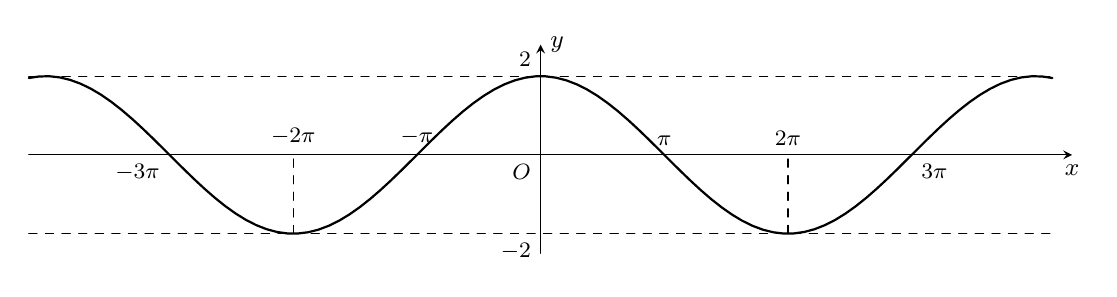
\begin{tikzpicture}[>=stealth,line join=round,line cap=round,font=\footnotesize,scale=0.5]
					\draw[->] (-13,0) -- (13.5,0) node[below] {\small $x$};
					\draw[->] (0,-2.5) -- (0,2.8) node[right] {\small $y$};
					\draw[thick,samples=100,domain=-13:13] plot(\x,{2*cos((\x)*90/pi)});
					\draw (0,0) node [below left] {$O$};
					\draw (0,2) node [above left] {$2$};
					\draw (0,-2) node [below left] {$-2$};
					\draw (-pi,0) node[above] {$-\pi$};
					\draw (pi,0) node[above] {$\pi$};
					\draw[dashed] (-2*pi,-2)--(-2*pi,0) node[above] {$-2\pi$};
					\draw[dashed] (2*pi,-2)--(2*pi,0) node[above] {$2\pi$};
					\draw (-3*pi,0) node[below left] {$-3\pi$};
					\draw (3*pi,0) node[below right] {$3\pi$};
					\draw[dashed] (-13,2)--(13,2);
					\draw[dashed] (-13,-2)--(13,-2);
				\end{tikzpicture}
			\end{center}
\choice
{\True $y=2\cos \dfrac{x}{2}$}
{$y=\sin x+2$}
{$y=2\sin \dfrac{x}{2}$}
{$y=1+2\cos x$}
\loigiai{
Thử điểm $\left( 0\,;\,1 \right)$ lần lượt vào các hàm số $y=2\cos \dfrac{x}{2}$, $y=\sin x+2$, $y=2\sin \dfrac{x}{2}$, $y=1+2\cos x$ thấy rằng điểm $\left( 0\,;\,1 \right)$ không thuộc vào đồ thị hai hàm số $y=2\sin \dfrac{x}{2}$ và $y=1+2\cos x$.\\
Thử điểm $\left( \pi \,;\,0 \right)$ vào hai hàm số $y=2\cos \dfrac{x}{2}$, $y=\sin x+2$ thấy rằng điểm $\left( \pi \,;\,0 \right)$ hông thuộc vào đồ thị hàm số $y=1+2\cos x$.\\
Vậy hình vẽ chỉ có thể là đồ thị hàm số $y=2\cos \dfrac{x}{2}$.}
\end{ex}
\Closesolutionfile{ans}
\indapan{6}{ans/ans-11-C1B4-DE2-LC}

\Opensolutionfile{ans}[ans/ans-11-C1B4-DE2-DS]
\cauds
%%%==============EX_15============%%%
\begin{ex}%[1D1N4-5]
	Cho các hàm số $f(x)=\sqrt{3-2\sin x}$; và $g(x)=\tan \dfrac{x}{2}-\dfrac{1}{3} \cos x$, khi đó:
	\choiceTF
		{\True Hàm số $f(x)$ có tập xác định là $\mathscr{D}=\mathbb{R}$}
		{\True Hàm số $f(x)$ đã cho là hàm tuần hoàn}
		{Hàm số $g(x)$ xác định khi $x\ne k2\pi, (k\in \mathbb{Z})$}
		{Hàm số $g(x)$ đã cho là hàm không tuần hoàn}
	\loigiai{
	\begin{itemchoice}
		\itemch Đúng. Hàm số xác định $\Leftrightarrow 3-2\sin x\ge 0\Leftrightarrow \sin x\le \dfrac{3}{2}$ (đúng với mọi $x\in \mathbb{R}$).
			
			Vì vậy tập xác định hàm số là $\mathscr{D}=\mathbb{R}$. 
		\itemch Đúng. Với mọi $x\in \mathscr{D}$ thì $x\pm 2\pi \in \mathscr{D}$ và $$f(x+2\pi)=\sqrt{3-2\sin (x+2\pi)}=\sqrt{3-2\sin x}=f(x).$$
			Vậy hàm số đã cho là hàm tuần hoàn.
		\itemch Sai. Hàm số xác định $\Leftrightarrow \cos \dfrac{x}{2} \ne 0\Leftrightarrow \dfrac{x}{2} \ne \dfrac{\pi}{2}+k\pi, (k\in \mathbb{Z})\Leftrightarrow x\ne \pi+k2\pi (k\in \mathbb{Z})$.
			
			Vì vậy tập xác định hàm số là $\mathscr{D}=\mathbb{R}\setminus \{\pi+k2\pi k\in \mathbb{Z}\}$.
			
		\itemch Sai. Với mọi $x\in \mathscr{D}$ thì $x\pm 2\pi \in \mathscr{D}$ và
			\[\begin{array}{ll} {f(x+2\pi)} & {=\tan \dfrac{x+2\pi}{2}-\dfrac{1}{3} \cos (x+2\pi)} \\ {} & {=\tan \left(\dfrac{x}{2}+\pi \right)-\dfrac{1}{3} \cos x=\tan \dfrac{x}{2}-\dfrac{1}{3} \cos x=f(x).} \end{array}
			\]
			Vậy hàm số đã cho là hàm tuần hoàn.
		\end{itemchoice}
			}
\end{ex}
%%%==============EX_17============%%%
\begin{ex}%[1D1N4-4]
	Cho các hàm số sau: $f(x)=2\cos 3x-1$; $g(x)=|2\sin x+2|+|2\sin x-2|$. Khi đó
	\choiceTF
		{\True Tập xác định hàm số $f(x)$ là $\mathscr{D}=\mathbb{R}$}
		{\True Hàm số $f(x)$ đã cho là hàm số chẵn}
		{\True Tập xác định hàm số $g(x)$ là $\mathscr{D}=\mathbb{R}$}
		{Hàm số $g(x)$ đã cho là hàm số lẻ}
	\loigiai{
	\begin{itemchoice}
		\itemch Đúng. Xét $y=f(x)=2\cos 3x-1$
			
			Tập xác định $\mathscr{D}=\mathbb{R}$ suy ra $\forall x\in \mathscr{D}$ thì $-x\in \mathscr{D}$.
			
		\itemch	Đúng. Ta có $f(-x)=2\cos (-3x)-1=2\cos 3x-1=f(x)$.
			
			Do đó hàm số đã cho là hàm số chẵn.
		\itemch Đúng. Xét $y=f(x)=|2\sin x+2|+|2\sin x-2|$
			
			Tập xác định $\mathscr{D}=\mathbb{R}$ suy ra $\forall x\in \mathscr{D}$ thì $-x\in \mathscr{D}$.
			
		\itemch	Sai. Ta có 
$$
\begin{aligned}
f(-x)&=|2\sin (-x)+2|+|2\sin (-x)-2|=|-2\sin x+2|+|-2\sin x-2|\\
 &=|-2\sin x+2|+|-2\sin x-2|=|2\sin x-2|+|2\sin x+2|=f(x).
\end{aligned}
$$			
			Do đó hàm số đã cho là hàm số chẵn.
		\end{itemchoice}
			}
\end{ex}
%%%==============EX_19============%%%
\begin{ex}%[1D1H4-2]
	Tìm được tập xác định các hàm số sau. Khi đó
	\choiceTF
		{\True Hàm số $y=\tan \left(x-\dfrac{\pi}{2} \right)$ xác định $\Leftrightarrow \cos \left(x-\dfrac{\pi}{2} \right)\ne 0$}
		{\True Hàm số $y=\dfrac{1+\cos x}{\sin x}$ có tập xác định là $\mathscr{D}=\mathbb{R}\setminus \{\left. k\pi \right|k\in \mathbb{Z}\}$}
		{\True Hàm số $y=\cot \left(3x-\dfrac{\pi}{4} \right)$ xác định $x\ne \dfrac{\pi}{12}+\dfrac{k\pi}{3} (k\in \mathbb{Z})$}
		{Hàm số $y=\dfrac{\cot x}{\sqrt{3} \tan x-3}$ xác định $\Leftrightarrow \left\{\begin{array}{l} {\sin x\ne 0} \\ {\cos x\ne 0} \end{array}\right.$}
	\loigiai{
	\begin{itemchoice}
		\itemch Đúng. Hàm số $y=\tan \left(x-\dfrac{\pi}{2} \right)$ xác định 
		
		$\Leftrightarrow \cos \left(x-\dfrac{\pi}{2} \right)\ne 0\Leftrightarrow x-\dfrac{\pi}{2} \ne \dfrac{\pi}{2}+k\pi (k\in \mathbb{Z})\Leftrightarrow x\ne \pi+k\pi (k\in \mathbb{Z}).$
		
			Vậy tập xác định của hàm số $\mathscr{D}=\mathbb{R}\setminus \{\pi+k\pi k\in \mathbb{Z}\}$.
		\itemch Đúng. Hàm số $y=\dfrac{1+\cos x}{\sin x}$ xác định $\Leftrightarrow \sin x\ne 0\Leftrightarrow x\ne k\pi (k\in \mathbb{Z})$.
			
			Vậy tập xác định của hàm số $\mathscr{D}=\mathbb{R}\setminus \{\left. k\pi \right|k\in \mathbb{Z}\}$.
		\itemch Đúng. Hàm số $y=\cot \left(3x-\dfrac{\pi}{4} \right)$ xác định $\Leftrightarrow 3x-\dfrac{\pi}{4} \ne k\pi \Leftrightarrow x\ne \dfrac{\pi}{12}+\dfrac{k\pi}{3} (k\in \mathbb{Z})$.
			
			Vậy tập xác định của hàm số $\mathscr{D}=\mathbb{R}\setminus \left\{\dfrac{\pi}{12}+\dfrac{k\pi}{3} \left|k\in \mathbb{Z}\right. \right\}$.
		\itemch Sai. Hàm số $y=\dfrac{\cot x}{\sqrt{3} \tan x-3}$ xác định $\Leftrightarrow \left\{\begin{array}{l} {\sin x\ne 0} \\ {\cos x\ne 0} \\ {\sqrt{3} \tan x-3\ne 0} \end{array}\right.$
			
			Vậy tập xác định của hàm số $\mathscr{D}=\mathbb{R}\setminus \left\{\dfrac{k\pi}{2}, \dfrac{\pi}{3}+k\pi k\in \mathbb{Z}\right\}$.
	\end{itemchoice}
			}
\end{ex}
%%%==============EX_22============%%%
\begin{ex}%[1D1H4-6]
	Cho hàm số $y=3-\sin \left(2x+\dfrac{\pi}{4} \right)$, khi đó
	\choiceTF
		{\True Hàm số có tập xác định $\mathscr{D}=\mathbb{R}$}
		{\True Giá trị nhỏ nhất của hàm số bằng $2$}
		{\True Giá trị lớn nhất của hàm số bằng $4$}
		{\True Tập giá trị của hàm số là $T=[2;4]$}
	\loigiai{
	\begin{itemchoice}
		\itemch Đúng. Ta có hàm số có tập xác định $\mathscr{D}=\mathbb{R}$.
		\itemch Đúng. Ta có 
$$
\begin{aligned}
-1\le \sin \left(2x+\dfrac{\pi}{4} \right)\le 1 &\Leftrightarrow 1\ge-\sin \left(2x+\dfrac{\pi}{4} \right)\ge-1 \\
& \Leftrightarrow 4\ge 3-\sin \left(2x+\dfrac{\pi}{4} \right)\ge 2\Leftrightarrow 4\ge y\ge 2.
\end{aligned}
$$	
		\itemch Đúng. Ta có hàm số có tập xác định $\mathscr{D}=\mathbb{R}$.
		$$
\begin{aligned}
-1\le \sin \left(2x+\dfrac{\pi}{4} \right)\le 1 &\Leftrightarrow 1\ge-\sin \left(2x+\dfrac{\pi}{4} \right)\ge-1\\
& \Leftrightarrow 4\ge 3-\sin \left(2x+\dfrac{\pi}{4} \right)\ge 2\Leftrightarrow 4\ge y\ge 2.
\end{aligned}
$$	
		\itemch Đúng. Vì $4\ge y\ge 2$ nên giá trị của hàm số là $T=[2;4]$.
	\end{itemchoice}
		}
\end{ex}
\Closesolutionfile{ans}
\indapan{3}{ans/ans-11-C1B4-DE2-DS}

\Opensolutionfile{ans}[ans/ans-11-C1B4-DE2-KQ]
\caukq
%%%==============EX_16============%%%
\begin{ex}%[1D1H4-6]
Tìm giá trị nhỏ nhất của hàm số $y=\sqrt{1+\sin x}-3$.
	
	\shortans{$-3$}
\loigiai{
	\[y=f(x)=\sqrt{1+\sin x}-3.
	\]
	Do $\sin x\ge-1,\forall x\in \mathbb{R}$ nên tập xác định của hàm số là $\mathscr{D}=\mathbb{R}$.\\
	Ta có $-1\le \sin x\le 1,\forall x\in \mathbb{R}$ nên $\sqrt{1+\sin x}-3\ge -3$.
	}
\end{ex}
%%%==============EX_17============%%%
\begin{ex}%[1D1H4-6]
Tìm giá trị lớn nhất của hàm số $y=2+2\cos x+\cos^2 x$.
	
	\shortans{$3$}
\loigiai{
	\[y=f(x)=2+2\cos x+\cos^2 x=(\cos x+1)^2+1
	\]
	Vì $-1\le \cos x\le 1,\forall x\in \mathbb{R}$ nên $0\le 1+\cos x\le 2,\forall x\in \mathbb{R}\Rightarrow 1\le (1+\cos x)^2+1\le 3,\forall x\in \mathbb{R}\Rightarrow 1\le f(x)\le 3,\forall x\in \mathbb{R}$. Do đó
	\[\begin{array}{l} {f_{\min\;} (x)=1\Leftrightarrow \cos x=-1\Leftrightarrow x=\pi+k2\pi, k\in \mathbb{Z}.} \\ {f_{\max\;} (x)=3\Leftrightarrow \cos x=1\Leftrightarrow x=k2\pi, k\in \mathbb{Z}.} \end{array}
	\]
	}
\end{ex}
%%%==============EX_18============%%%
\begin{ex}%[1D1H4-6]
Tìm $x\in \left[\pi;2\pi\right]$ để hàm số $y=1-3\sqrt{1-\cos^2 x}$ đạt giá trị nhỏ nhất (kết quả làm tròn đến hàng phần mười).\shortans{$4,7$}
\loigiai{
	Ta có $\cos^2 \ge 0\Rightarrow-\cos^2 \le 0\Leftrightarrow 1-\cos^2 \le 1$
	\[\begin{array}{l} {\Rightarrow \sqrt{1-\cos^2} \le 1\Leftrightarrow-3\sqrt{1-\cos^2} \ge-3\Leftrightarrow 1-3\sqrt{1-\cos^2} \ge-2} {\Leftrightarrow y\ge-2.} \end{array}
	\]
	(Dấu \lq\lq = \rq\rq xảy ra $\Leftrightarrow 1-\cos^2 x=1\Leftrightarrow \cos^2 x=0\Leftrightarrow \dfrac{1+\cos 2x}{2}=0$
	\[ \Leftrightarrow \cos 2x=-1\Leftrightarrow 2x=\pi+k2\pi, k\in \mathbb{Z}\Leftrightarrow x=\dfrac{\pi}{2}+k\pi, k\in \mathbb{Z}.)
	\]
	Vậy tại $x=\dfrac{\pi}{2}+k\pi, k\in \mathbb{Z}$ thì $y$ đạt giá trị nhỏ nhất bằng $-2$. Vì $x\in \left[\pi;2\pi\right]$ nên $x=\dfrac{3\pi}{2}\approx 4,7$.
	}
\end{ex}
%%%==============EX_20============%%%
\begin{ex}%[1D1V4-2]
Tìm số các giá trị nguyên của tham số $m$ để hàm số $y=\sqrt{\dfrac{m-1}{m}-2\cos 4x}$ xác định trên $\mathbb{R}$.\shortans{$1$}
\loigiai{
	Để hàm số $y=\sqrt{\dfrac{m-1}{m}-2\cos 4x}$ xác định trên $\mathbb{R}$.
	$${\begin{aligned}
\frac{m-1}{m}-2 \cos 4 x \geq 0, \forall x \in \mathbb{R} \Leftrightarrow \frac{m-1}{2 m} \geq \cos 4 x \geq 1  \Leftrightarrow \frac{m-1}{2 m} \geq 1 \Leftrightarrow-1 \leq m < 0.
\end{aligned}
}$$
Vì $m$ là số nguyên nên $m\in\{-1\}$.
	}
\end{ex}
%%%==============EX_22============%%%
\begin{ex}%[1D1H4-6]
Tìm tổng bình phương giá trị lớn nhất và giá trị nhỏ nhất của hàm số $y=\sin x+\cos x$. \shortans{$4$}
\loigiai{
  $$y=\sin x+\cos x=\sqrt{2} \sin x\cdot \cos \dfrac{\pi}{4}+\sqrt{2} \cos x\cdot \sin \dfrac{\pi}{4}=\sqrt{2} \sin \left(x+\dfrac{\pi}{4} \right).$$
$-1\le \sin \left(x+\dfrac{\pi}{4} \right)\le 1,\forall x\Leftrightarrow-\sqrt{2} \le y\le \sqrt{2}$. Suy ra $y_{min\;}=-\sqrt{2}$ và $y_{\max}=\sqrt{2}$.\\
Do đó $y_{min}^2+y_{\max}^2=4$.
	}
\end{ex}
%%%==============EX_23============%%%
\begin{ex}%[1D1H4-5]
Tính chu kỳ hàm số $y=\cos 3x$ (kết quả làm tròn đến hàng phần mười).

	\shortans{$2,1$}
\loigiai{
Tập xác định $\mathscr{D}=\mathbb{R}$. Ta có $x\in \mathscr{D}\Rightarrow x\pm \dfrac{2\pi}{3} \in \mathscr{D}$ và
\[f\left(x+\dfrac{2\pi}{3} \right)=\cos \left[3\left(x+\dfrac{2\pi}{3} \right)\right]=\cos (3x+2\pi)=\cos 3x=f(x).
\]
Vậy $f(x)$ là hàm số tuần hoàn với $T=\dfrac{2\pi}{3}\approx 2,1$.} 
\end{ex}
\Closesolutionfile{ans}
\indapan{3}{ans/ans-11-C1B4-DE2-KQ}